% Chapter 2

\chapter{Basic Theory of Optical Coherence Tomograpy} % Chapter title
\label{ch:theory} % For referencing the chapter elsewhere, use \autoref{ch:examples} 

In this chapter I will report the basic theoretical background needed to comprehend the working mechanisms behind the OCT technique, introduce the different schemes and compare them in terms of performance. The content of this chapter is partially adapted from \cite{Midrio2006,Someda2006,Wolf1999}. 


\section{Principles of Coherence and Interference}
A solution to a generic electromagnetic problem is completely determined by the vector couple $\mathcal{S} = \left\{\mathbf{E}(\mathbf{r}, t),\; \mathbf{H}(\mathbf{r}, t)\right\}$, whose components represent the time-varying electric and magnetic field, respectively ($\textbf{r}$ is the three-dimensional vector determining the position in space at which the field is evaluated). The electromagnetic field determined by $\mathcal{S}$ is considered a valid solution if it satisfies both Maxwell's Equations and the boundary conditions specific to the problem. 

For monochromatic waves, i.e. fields oscillating at a single frequency $\omega$, we can use Steinmetz notation and write
\begin{equation}\label{eq:steinmetz}
	\textbf{E}(\textbf{r}, t) = \Re\left[\widetilde{\mathbf{E}}(\textbf{r})e^{j\omega t}\right] \qquad \textbf{H}(\textbf{r}, t) = \Re\left[\widetilde{\mathbf{H}}(\textbf{r})e^{j\omega t}\right]\,,
\end{equation}
where $\widetilde{\textbf{E}}$ and $\widetilde{\textbf{H}}$ are complex 3D vectors and $\Re\left[\cdot\right]$ is the real value operator. Maxwell Equations can then be rewritten in the frequency domain. In a linear, homogeneous, isotropic, and current-free medium, Maxwell's equations can be written in the following way

\begin{subequations}\label{eq:maxwell-frequency}
\begin{align}
& \nabla \times \widetilde{\textbf{E}} = -j\omega\mu\widetilde{\textbf{H}} \label{eq:maxwell-e}\\
& \nabla \times \widetilde{\textbf{H}} = j\omega\varepsilon_c\widetilde{\textbf{E}}\label{eq:maxwell-h}
\end{align}
\end{subequations}
where $\mu$ is the magnetic permeability of the medium, $\varepsilon_c = \varepsilon - \sigma/\omega$ is the complex dielectric permettivity. The simplest solution of \autoref{eq:maxwell-frequency} is given by the \emph{homogeneous plane wave}. Using a cartesian coordinate system, the electric field can be expressed as
\begin{equation}\label{eq:e-field-expansion}
		\widetilde{\textbf{E}}(\textbf{r}) = \sum_{i=1}^3 A_i \cdot \hat{\textbf{x}}_i  = \sum_{i=1}^3 a_i \exp\left[jg_i(\textbf{r})\right]  \cdot \hat{\textbf{x}}_i
\end{equation}
where the amplitudes $a_i$ are constant and $g_i(\textbf{r}) = \textbf{k}\cdot\textbf{r} - \delta_i$ represent the phase functions of the electric field components. The propagation vector $\textbf{k}$ is given as a function of the wavelength $\lambda$ as follows
\begin{equation}
	|\textbf{k}| = \frac{2\pi}{\lambda},
\end{equation}
while the $\delta_i$'s are the phase differences which determine the state of polarization of the electromagnetic field. The magnetic field is instead obtained by applying \autoref{eq:maxwell-e} to \autoref{eq:e-field-expansion}. 

The intensity of an electromagnetic field is given by the time average of the amount of energy which crosses in a unit time a unit area perpendicular to the direction of the energy flow. In the case of homogenous plane waves, it is expressed as
\begin{equation}\label{eq:intensity}
	I \propto \langle \textbf{E}^2 \rangle
\end{equation}

Using \autoref{eq:steinmetz}, we can express the electric field as
\begin{equation}\label{eq:e-steinmetz}
\textbf{E}(\textbf{r}, t) = \frac{1}{2}\left[ \widetilde{\textbf{E}}(\textbf{r})e^{-j\omega t} + \widetilde{\textbf{E}}^*(\textbf{r})e^{j\omega t}\right],
\end{equation}
so that \autoref{eq:intensity} can be written as
\begin{equation}
	\langle\textbf{E}^2\rangle = \frac{1}{4} \left\langle\widetilde{\textbf{E}}^2 e^{-2j\omega t} + \widetilde{\textbf{E}}^{*2}e^{2j\omega t} + 2  \widetilde{\textbf{E}}\cdot\widetilde{\textbf{E}}^*\right\rangle \,.
\end{equation}
Averaging over a time interval sufficiently larger than the period $T=2\pi/ \omega$, we obtain
\begin{equation}
	\langle \textbf{E}^2 \rangle =\frac{1}{2}\widetilde{\textbf{E}}\cdot\widetilde{\textbf{E}}^* =\frac{1}{2}\left(a_1^2 + a_2^2 + a_3^2\right) = \text{constant},
\end{equation}
as the high frequency terms at $2\omega$ are canceled by the detector.

Suppose now that the field $\textbf{E}$ is split in two components $\textbf{E}_1$ and $\textbf{E}_2$ which are then superimposed in a certain point $\textbf{r}'$ in space, then

\begin{equation}
\textbf{E}(\textbf{r}') = \textbf{E}_1(\textbf{r}') + \textbf{E}_2(\textbf{r}'),
\end{equation}

which implies that
\begin{equation}
	\textbf{E}^2 (\textbf{r}')= \textbf{E}_1^2(\textbf{r}') + \textbf{E}_2^2(\textbf{r}') + 2\textbf{E}_1(\textbf{r}')\cdot\textbf{E}_2(\textbf{r}')
\end{equation}

The field intensity is thus
\begin{equation}\label{eq:intensity-interference}
I = I_1 + I_2 + J_{12} = \langle\textbf{E}_1^2\rangle + \langle\textbf{E}_2^2\rangle + 2\langle\textbf{E}_1\cdot\textbf{E}_2\rangle.
\end{equation}
The last term in \autoref{eq:intensity-interference} is called \emph{interference}. Depending on the phase difference between the two fields, the total intensity can assume different values.  If the difference between the optical paths traveled by the two components is $\Delta z$, the phase difference will be $\delta = \Delta z \cdot 2\pi/\lambda $, and the interference term will be equal to
\begin{equation}
	J_{12} = 2\langle\textbf{E}_1\cdot\textbf{E}_2\rangle = \left(a_1^2 + a_2^2 + a_3^2\right)\cos\delta.
\end{equation}
In the simple case in which the two fields are linearly polarized along the $\textbf{x}_1$ direction, we have that $a_2 = a_3 = 0$, and $I_1 = I_2 = 1/2\, a_1^2$, while the interference is
given by $J_12 = a_1^2\cos\delta = 2\sqrt{I_1 I_2}\cos \delta$. 
The total intensity is then
\begin{equation}
	I = I_1 + I_2 + 2 \sqrt{I_1I_2}\cos\delta = 2I_1 + 2I_1\cos\delta \in [0, 4I_1].
\end{equation}
The intensity profile is displayed in \autoref{fig:intensity-interference}. In this first approximation of perfectly monochromatic waves there are no constraint on the phase offset $\delta$ or on the optical path difference $\Delta z$ for the presence of intereference. 

\begin{figure}[hbt]
	\myfloatalign
	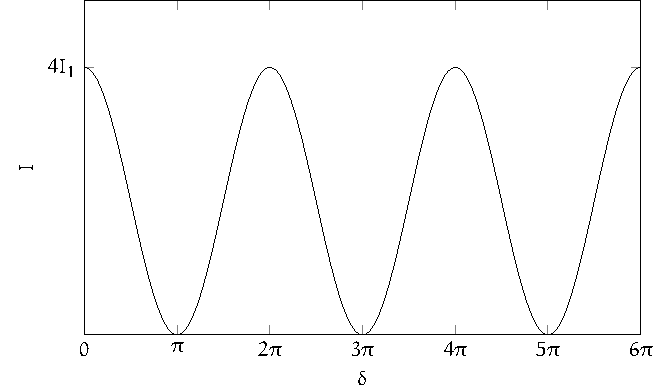
\includegraphics[]{gfx/tikz/interference.pdf}
	\caption{Interference fringes created by two beams of equal intensity.}\label{fig:intensity-interference}
\end{figure}

\subsection{Michelson interferometer}
\label{sub:michelson}
A classical example of the application of interference is given by the scheme called \emph{Michelson interferometer}. In \autoref{fig:michelson} the schematic diagram of the interferometer is given. A light source emits an electric field $\textbf{E}_0$ which is then split in two by a semitransparent mirror. The two replicas, $\textbf{E}_1$ and $\textbf{E}_2$, travel along the two \emph{arms} of the interferometer, of length $l_1$ and $l_2$, are reflected by two mirrors and finally recombined. The intensity of the superposition of two fields is then measured by a photodetector. The two replicas arrive at the detector with a time difference given by
\begin{equation}
	\tau = 2\frac{l_2 - l_1}{c},
\end{equation}
where $c$ is the speed of light in the considered medium. From \autoref{eq:intensity-interference} we then obtain
\begin{align}\label{eq:michelson-intensity}
	I &= I_1 + I_2 + 2 \langle\textbf{E}_1(t) \cdot \textbf{E}_2(t)\rangle =  2 \left[I_1 + \langle\textbf{E}_1(t) \textbf{E}_1(t-\tau) \rangle\right]\\
	 &= 2I_1\left\{ 1 + \cos\left[\frac{2\pi}{\lambda}2(l_2-l_1)\right]\right\}.
\end{align}

%\todo{Expand this formula defining the degree of coherence so that it's easier to describe TDOCT signals}

\begin{figure}[hbt]
	\myfloatalign
	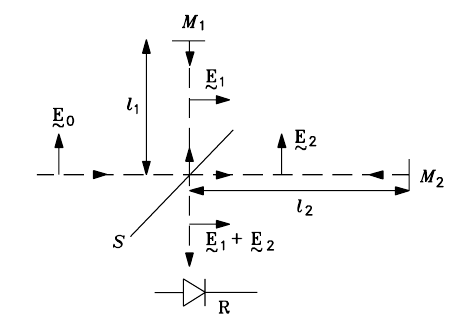
\includegraphics[width=0.7\linewidth]{gfx/michelson}
	\caption{Diagram of a Michelson interferometer \cite{Someda2006}. }\label{fig:michelson}
\end{figure}

This type of interferometer can be used to perform high-precision measurements of distances by making one of the arms mobile and mantaining the other fixed as a reference. Counting the number of "peaks" and "valleys" of the intensity profile as the mobile arm is translated, an estimate of path length difference is given with a precision of $\lambda/2$. \\


\subsection{Fringe visibility}

\noindent We can define a useful parameter called \emph{fringe visibily} as follows
\begin{equation}
\label{eq:fringevisibily}
v = \frac{I_{max} - I_{min}}{I_{max} + I_{min}}.
\end{equation}


For a perfectly monochromatic source, $v$ will always be constant. In particular, in the case when $I_1 = I_2$  $v$ is equal to 1, as $I_{min} = 0$. Real-life optical sources however will always have a bandwidth $\Delta f$ greater than 0. In these cases $v$ is a monotonically decreasing function of the time delay $\tau$.  The \emph{coherence time} of a source is defined as the value $\tau_c$ such that $v(\tau_c) = 1/e$ (\autoref{fig:fringe-visibility}). 




\begin{figure}[hbt]
	\myfloatalign
	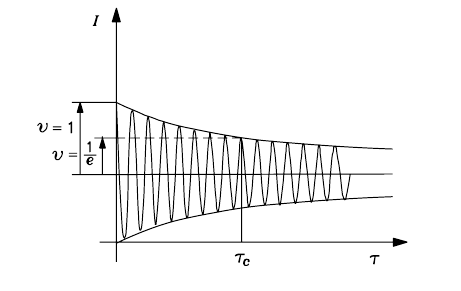
\includegraphics[width=0.8\linewidth]{gfx/fringe-visibility}
	\caption{Effect of the coherence time of a source on the interference fringes at the output of a Michelson interferometer \cite{Someda2006}.}\label{fig:fringe-visibility}
\end{figure}


Intuitively, we may think of the coherence time as the time slot after which the optical source loses memory of what it was at the beginning. In fact, after this time slot has passed, some properties of the source randomly change due to the stochastic nature of photon emission. A perfectly coherent source emits a sinusoidal field with a well defined and constant phase relation. Similarly, two electromagnetic fields are perfectly coherent if the phase difference between the two is mantained constant for an infinite amount of time. This property is however impossible to obtain in real life, as every source has a finite coherence time. This concept is explained by the uncentainty-principle, which states that 
\begin{equation}
	\tau_c \geq \tau_{min} = \frac{1}{\mathcal{B}},
\end{equation}
where $\mathcal{B}$ is the bandwidth of the source. This equation results in the fact that there are no sources which are completely incoherent in time, as they would require an infinite bandwidth.

\subsection{The coherence function}
Another way to describe the coherence property of light other than the fringe visibility parameter, is through the so-called \emph{mutual coherence function}. It is defined for polychromatic, i.e., non-monochromatic fields as follows \cite{Wolf1999}:

\begin{equation}\label{eq:mutual-coherence}
	\Gamma_{12}(\tau) = \left\langle  \mathbf{E}_1(t+\tau)\mathbf{E}_2^*(t)   \right\rangle,
\end{equation}
If $\mathbf{E}_1 = \mathbf{E}_2$, it is called \emph{self-coherence function}, and it's written as $\Gamma_{11}(\tau)$. Notice that when $\tau = 0$ it reduces to the field intensity:
\begin{equation}
	\Gamma_{ii}(0) = I_i\,.
\end{equation}
It is then useful to apply the following normalization
\begin{equation}
	\gamma_{ij} (\tau) = \frac{\Gamma_{ij}(\tau)}{\sqrt{\Gamma_{ii}(0)}\sqrt{\Gamma_{jj}(0)}},
\end{equation}
so that it assumes values in the $[0,1]$ interval. This normalized function is called \emph{complex degree of coherence}, and it allows the following definitions:
\begin{enumerate}
	\item Completely incoherent fields: $|\gamma_{ij}| = 0$, no interference fringes are visible.
	\item Completely coherent fields: $|\gamma_{ij}| = 1$, the total intensity includes the interference term. 
	\item Partially coherent fields: $0 < |\gamma_{ij}| < 1$, interference fringes are present, and assume a visibility parameter equal to 
	\begin{equation}
		v = \frac{2\sqrt{I_i I_j}}{I_i + I_j}|\gamma_{ij}|.
	\end{equation}
	When the two fields have equal intensity, than the two parameters coincide.
\end{enumerate}

Using this notation, the equation for the intensity of two partially-coherent beams is then
\begin{equation}
	I = I_1 + I_2 + 2\sqrt{I_1I_2}|\gamma_{12}(\tau)| \cos( \delta )\,
\end{equation}
where we can clearly see the effect of coherence on the shaping of the interference fringes. Using the coherence function instead of the fringe visibility as a measure of coherence, the coherence time of a source, $\tau_c$, is defined as the \ac{FWHM} parameter of its self-coherence function, that is, the value of $\tau$ such that
\begin{equation}
	|\gamma(\tau)| = \frac{|\gamma(0)|}{2}.
\end{equation}

The shape of the coherence function of an optical source is completely determined by its spectrum $I(k)$ through the Wiener-Khintchine theorem, which states that the autocorrelation function and the \ac{PSD} of a random process are connected through their Fourier Transform. 




\subsection{Coherence length}

Starting from the coherence time of the source, $\tau_c$, we can also define its coherence length as follows
\begin{equation}
	l_c = c_0 \tau_c,
\end{equation}
where $c_0 \simeq 3\cdot10^8$ m/s is the speed of light in vacuum. Using a light source with a coherence length $l_c$ in the Michelson interferometer previously presented, we would observe an interference pattern at the photoreceiver only if the difference in length of the two arms is such that 
\begin{equation}
\Delta l = |l_2 - l_1| \leq l_c / 2,
\end{equation}
or, equivalently, if the total \ac{OPD} is matched to within the coherence length of the source. 


While we just defined the coherence \emph{length} of a source, it's important to note that it is a parameter that is directly related to the time coherence and does not describe the phenomenon of spatial coherence. 

\section{OCT Terminology}
Before introducing the different OCT techniques it is useful to introduce some terminology that will be used throughout this thesis. The most basic OCT measure is called A-scan (Axial-scan), which is a signal that represents the reflectivity of a sample as a function of depth. The amount of information carried by these measurements is limited, but can be used to perform thickness measurements if the structure of the sample is known a priori. 

 \begin{figure}[hbt]
	\myfloatalign
	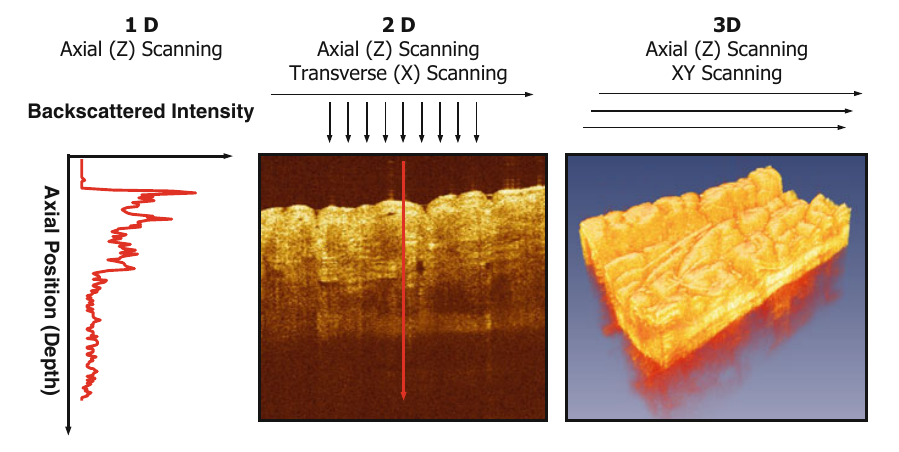
\includegraphics[width=\linewidth]{gfx/ch2/terminology}
	\caption{Diffent types of OCT measurements. \cite{Drexler2015}}\label{fig:terminology}
\end{figure}

If multiple consecutive A-scans are acquired along a transverse direction on the sample, a cross-sectional image, called B-scan, is generated. They are the most direct way to determine the anatomy of an unknown sample and are often sufficient for diagnostic purposes, especially in Ophtalmology. Their visualization does not require advanced techniques, but if a real-time high-resolution video stream is desired then careful design choices have to be made. 

Finally, 3D volumetric data can be generated by acquiring consecutive B-scans along a second direction on the transverse plane. Intuitively, they are called C-scans. Contrary to B-scans, volume rendering requires sophisticated and efficient algorithms for a correct data interpretation and visualization \cite{Lacroute1994,Cabral1994,Engel2001}. Starting from 3D data its also possible to obtain frontal projections of the sample, called \emph{en-face} views (\autoref{fig:enface}), or to generate cross-sections along an arbitrary plane.

 \begin{figure}[hbt]
	\myfloatalign
	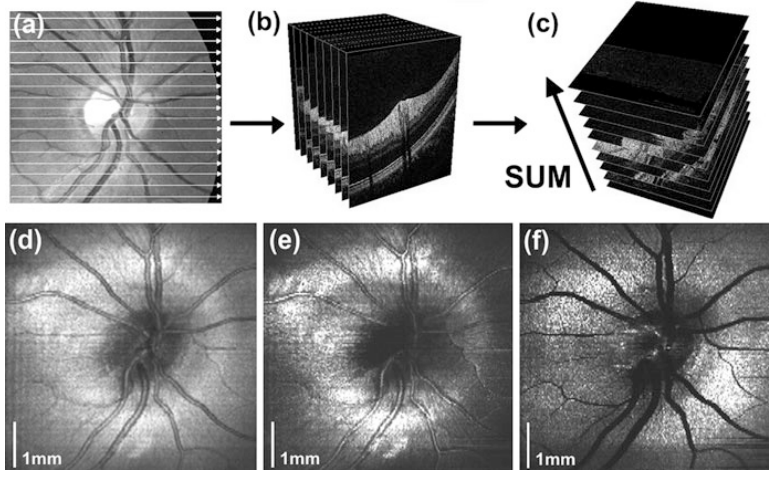
\includegraphics[width=\linewidth]{gfx/ch2/enface}
	\caption{\cite{Drexler2015}}\label{fig:enface}
\end{figure}

%The intensity profile given by \autoref{eq:michelson-intensity} can also be described through the \emph{coherence function} of the two fields, defined as
%\begin{equation}
%\Gamma_{ij}(\tau) = \left\langle  \textbf{E}_i(t)\cdot \textbf{E}_j(t+\tau)  \right\rangle,
%\end{equation}
%which gives
%\begin{equation}
%I = I_1 + I_2 + 2 \Re\left[\Gamma_{12}(\tau)\right] = I_1 + I_2 + 2 \Re\left[\Gamma_{21}(\tau)\right].
%\end{equation}
%
%In fact, since $\Gamma_{ii}(0) = I_i$, we can define the normalized coherence function as 
%\begin{equation}
%\gamma(\tau) = \frac{\Gamma(\tau)}{\Gamma(0)}
%\end{equation}




%In reality, eletromagnetic radiation consists in the emission of photons dictated by the decaying of atoms from a higher energy state to a lower energy state. The energy difference between these states, $E$, is directly proportional to the frequency $f$ of the emitted photon through Planck's constant $h$. The energy gap $E$ is however not uniquely defined, but is instead an interval of energies $\Delta E$, meaning that the frequency of the emitted photons will fall in a certain bandwidth $\Delta f = \Delta E / h$. 


%Copy from \cite{Wolf1999,Someda2006}

\section{Time Domain OCT}
 \acf{TD-OCT} was the first OCT technique that was demonstrated in the literature \cite{Huang1991}. The basic setup is that of a Michelson Interferometer in which one of the two mirrors is translatable and the other is replaced by the sample that we wish to analyze. The two arms are called respectively \emph{Reference arm} and \emph{Sample arm}. As explained in \autoref{sub:michelson}, the two beams arriving at the photodetector generate interference fringes if the \ac{OPD} is less than the coherence length $l_c$ of the source. A diagram of this setup is available in \autoref{fig:tdoct-michelson}. 
 
 
 \begin{figure}[hbt]
 	\myfloatalign
 	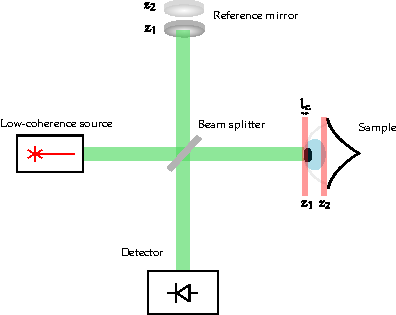
\includegraphics[width=0.8\linewidth]{gfx/tdoct}
 	\caption{Diagram of the basic \ac{TD-OCT} setup using a Michelson interferometer.}\label{fig:tdoct-michelson}
 \end{figure}
 
The light beam reflected by the reference mirror while in position $z_1$ will interfere with all the reflections occurring in the sample at depths $z \in [z_1 - l_c/2, z_1 + l_c/2]$. By measuring the intensity of the fringes it is then possible to obtain an estimate of the sample reflectivity at those depths. The whole axial measurement of the sample can be acquired by moving the translatable mirror along an adequate interval of positions. Since a single mirror position is mapped to an interval of length $l_c$ of axial positions in the sample, the coherence length of the source can be considered to be the axial resolution of the system. As a consequence short coherence lenghts are preferred, meaning that broadband sources are more widely employed. 

If the light source was perfectly monochromatic, the reference signal would interfere with an infinite number of reflected replicas generated at every depth in the sample, as there would be no constraint on the \ac{OPD}. 


To better understand this concept, suppose that the sample is an ideal reflector with a reflection coefficient $\rho_s$ is positioned in such a way that the \ac{OPD} is 0. The intensity measured by the detector when a \ac{OPD} equal to $\Delta z$ is introduced is then

\begin{align}\label{eq:tdoct-interference}
I(\Delta z) \propto |\rho_s|^2 |E_i|^2 + |\rho_r|^2 |E_i|^2 + |\rho_s\rho_r|^2|E_i|^2|\gamma(\Delta z)|\cos\left(\frac{2\pi}{\lambda_0}\Delta z\right)
\end{align}


\begin{figure}[hbt]
	\myfloatalign
	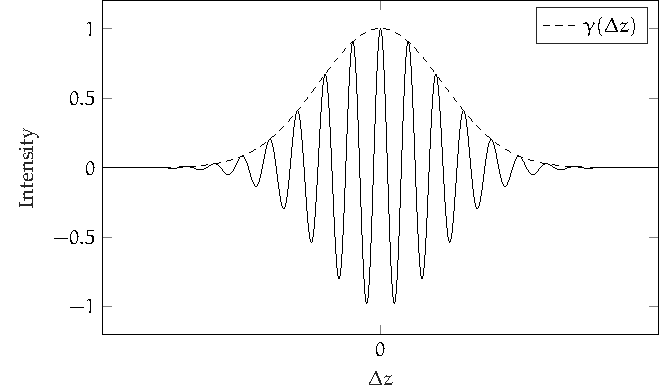
\includegraphics[width=0.8\linewidth]{gfx/tikz/tdoct-signal}
	\caption{Diagram of the basic \ac{TD-OCT} setup using a Michelson interferometer used in \cite{Huang1991}.}\label{fig:tdoct-signal}
\end{figure}


Apart from the DC offset given by the intensity of the two signals there is an oscillating term with period equal to $\lambda_0$, which is the central wavelength of the source. \autoref{fig:tdoct-signal} illustrates the oscillating term and its envelope, which is dictated by the coherence function $\gamma$ and the sample reflectivity $\rho_s$ (set equal to 1). With a perfectly coherent source $\gamma$ would be equal to 1 for all values of $\Delta z $ and we would not be able to identify the reflector. On the other hand, with an increasingly sharper $\gamma$, the ideal reflector would be more and more defined. 


Since the difference between the arm lengths is $\Delta l = \Delta z / 2$, when scanning the reference arm, interference fringes will be generated as a function of time with periodicity equal to $(\lambda/2) / \sigma$ where $\sigma$ is the scanning speed. 

 
\begin{figure}[hbt]
	\myfloatalign
	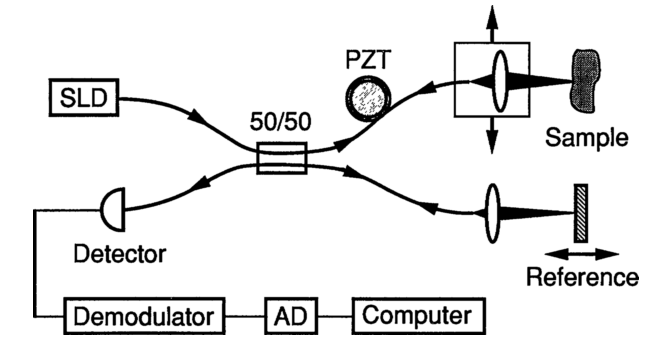
\includegraphics[width=0.8\linewidth]{gfx/ch2/huang-setup}
	\caption{Diagram of the basic \ac{TD-OCT} setup using a Michelson interferometer used in \cite{Huang1991}.}\label{fig:huang-setup}
\end{figure}

A setup similar to \autoref{fig:tdoct-michelson} can be created using fiber optics components and lenses to focus the optical beam on the sample and collect the reflections, as in \autoref{fig:huang-setup} \cite{Huang1991}. The role of splitting and recombining the signals is assigned to a fiber coupler, while a \ac{PZT} is used to frequency-modulate the interference signal and shift it inside the photodetector's bandwidth. The generated electrical signal is then filtered, demodulated and acquired by an \ac{ADC}.



\begin{figure}[hbt]
	\myfloatalign
	\subfloat[Optical ranging setup]
	{\label{fig:fujimoto-setup}
		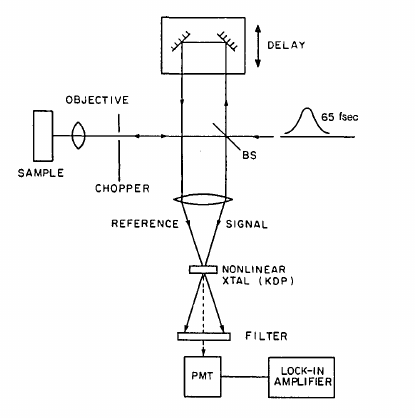
\includegraphics[width=0.45\linewidth]{gfx/ch2/fujimoto-setup}} \quad
	\subfloat[Lettuce leaf]
	{\label{fig:fujimoto-rabbit}
		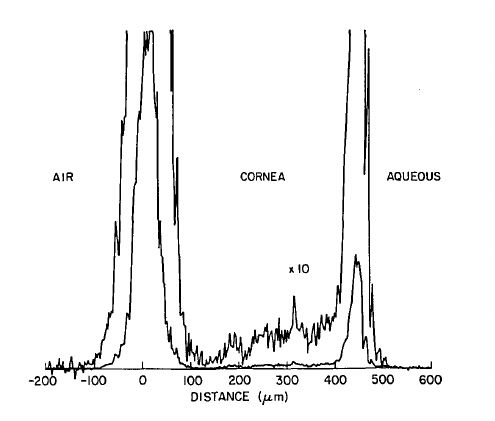
\includegraphics[width=0.45\linewidth]{gfx/ch2/fujimoto-rabbit}}\\
	\caption{ Optical ranging setup (left) and measurement (right) of the cornea of the rabbit eye \cite{Fujimoto1986}. }\label{fig:fujimoto}
\end{figure}

This imaging technique is also called \emph{Optical Ranging}, and was demonstrated by \citeauthor{Fujimoto1986}\cite{Fujimoto1986} in 1986. An A-scan of the cornea of a rabbit's eye was performed \emph{in vivo}, and is available in \autoref{fig:fujimoto-rabbit}. The peaks in signal intensity located at $l = 0$ and $l \sim 450$ $\mu$m are due to the strong reflection occurring at the interface between two different media. Inbetween these two peaks it's also possible to notice the effect of light scattered by the cornea, which is not present in the air and aqueous regions. 


To acquire B-scans and C-scans, axial measurements can be repeatedly performed while moving the sample on the orthogonal plane or by deflecting the impinging optical beam by means of galvanometric mirrors. 

The main disadvantage of this scheme is the slow acquisition rate, as it requires the mechanical movement of the reference arm. Consequently, \emph{in vivo} imaging is difficult to achieve since the movement of the sample could introduce heavy distortions on both B-scans and C-scans. 

\section{Fourier Domain OCT}
\label{sec:fdoct}
\acf{FD-OCT} is a group of OCT techniques that encode the depth information of a sample in the frequency content of the interference signal and decode it through a Fourier trasform operation. As opposed to \ac{TD-OCT}, an axial scan is obtained without the need of a scanning mirror in the reference arm. This results in a much faster acquisition speed and higher quality measurements, since the distortions caused by the mechanical vibrations and uncertainty on the position of the mirror are removed. On the other hand, \ac{FD-OCT} systems require more advanced laser sources and detection schemes, other than some numerical compensation and high speed \acp{ADC}. 


The two main \ac{FD-OCT} schemes are called \acf{SD-OCT} and \acf{SS-OCT}, and will be presented in the next sections. 

\begin{figure}[hbt]
	\myfloatalign
	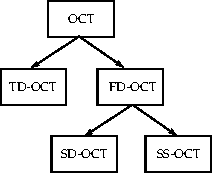
\includegraphics[width=0.5\linewidth]{gfx/ch2/oct-modalities}
	\caption{Diagram illustrating the different types of OCT modalities.}\label{fig:oct-modalities}
\end{figure}

\begin{figure}[hbt]
	\myfloatalign
	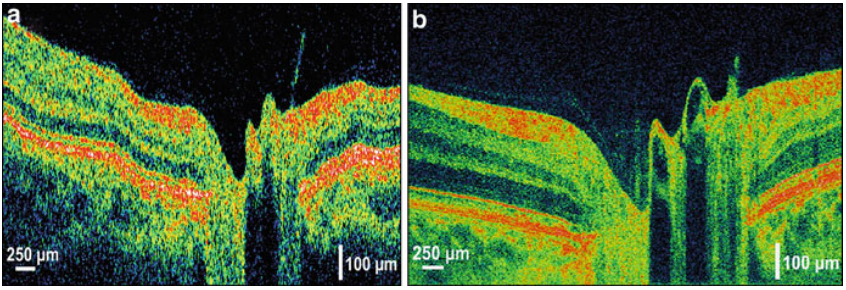
\includegraphics[width=0.95\linewidth]{gfx/ch2/td-fd-comparison}
	\caption{Comparison between images of the human retina obtained with standard \ac{TD-OCT} (left) and high-speed, high-resolution \ac{FD-OCT} (right).}\label{fig:td-fd-comparison}
\end{figure}

\subsection{Spectral Domain OCT}
\ac{SD-OCT} was the first type of \ac{FD-OCT} to be implemented, and was proposed by \citeauthor{Wojtkowski2002} in 2002 \cite{Wojtkowski2002}. This technique uses a \ac{SLD} as a broadband optical source, a Michelson interferometer similar to that in \autoref{fig:tdoct-michelson} and a detector consisting of a spectrometer. A diagram of the setup is available in \autoref{fig:fdoct-setup}. As already mentioned in \autoref{sec:fdoct}, \ac{SD-OCT} can acquire an A-scan with a single optical pulse, without the need to select the imaging depth through a scanning reference mirror. This comes at the price of a more complex detection scheme and the need for computationally intensive post-processing solutions. In order to achieve real-time performances, \ac{SD-OCT} scheme typically require the use of fast \acp{GPU}. 

\begin{figure}[hbt]
	\myfloatalign
	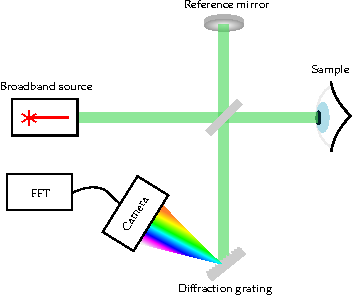
\includegraphics[width=0.75\linewidth]{gfx/ch2/fdoct-setup}
	\caption{}\label{fig:fdoct-setup}
\end{figure}


To gain insight on the working principle of \ac{SD-OCT}, we can rewrite \autoref{eq:tdoct-interference} as a function of the wavenumber $k = 2\pi/\lambda$ and fixing the \ac{OPD}:
\begin{equation}
	I(k) \propto I_{source}(k)\cos\left(k \Delta z\right)
\end{equation}
This means that a reflector placed at a depth $d = \Delta z/2$ will frequency modulate the source spectrum with a frequency that is linearly dependant on $d$. This effect is illustrated in \autoref{fig:fdoct-spectrum} for a broadband source centered at 1310 nanometers, with ideal reflectors positioned at $d_1 = \Delta z/2 = 12.5$ $\mu$m and $d_2 = \Delta z/2 = 25$ $\mu$m. 

\begin{figure}[hbt]
	\myfloatalign
	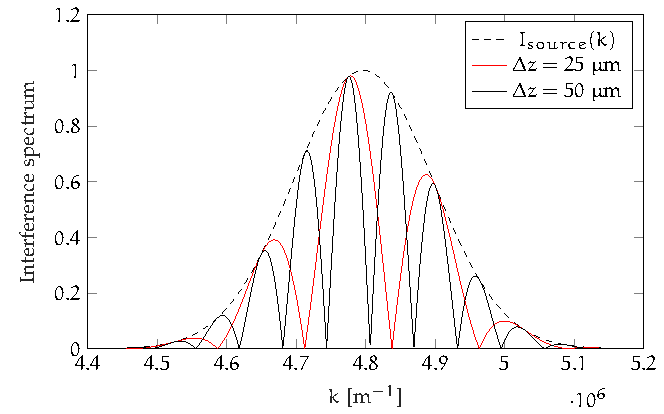
\includegraphics[width=0.85\linewidth]{gfx/tikz/fdoct-spectrum}
	\caption{}\label{fig:fdoct-spectrum}
\end{figure}

Using a diffraction grating or a prism, the spectrum of the interference signal is spatially separated and acquired through a linear photodetector, typically a \ac{CCD} or \ac{CMOS} camera. The corresponding A-scan is then computed using an inverse Fourier Transform operation, mapping modulation frequency in axial position. The depth of the various layers of the sample are encoded in the modulation frequency of the spectrum, while their reflectivity is encoded in the fringe visibility. 

A key observation has to be made regarding the role of the coherence function $\gamma$. In fact, the spectrum modulation induced by a reflection at depth $d=\Delta z /2$ can only be detected if $\gamma(d/2)$ is non-zero, that is, only the portion of the sample that is within the coherence length of the source can be imaged. This is the main disadvantage compared to \ac{TD-OCT} schemes, in which the depth of focus in the sample was selected with the mechanical movement of the reference mirror.


\subsubsection{Drawbacks}

\paragraph{Sampling distortion}
One of the major problems corcerning this detection technique is that the interference spectrum is usually detected linearly in the wavelength. For example, a diffraction grating spatially separates the different wavelengths at an angle $\beta_m$ with respect to the axis normal to the grating such that
\begin{equation}
	\sin\beta_m = m \frac{\lambda}{\Lambda} + \sin\alpha,
\end{equation}
where $\Lambda$ is the spacing between each line of the grating, $\alpha$ is the angle of the inpinging wave and $m$ is the order of diffraction. 
This behaviour requires a re-sampling of the acquired spectrum before computing the Fourier Transform in order to obtain a signal which is linearly spaced in frequency instead of wavelength. If this post-processing step is ignored, an oscillating term with a fixed frequency $\propto \Delta z$ in the interference spectrum will result in a broadened peak in the Fourier domain, as can be observed in \autoref{fig:fdoct-resampling}. The linear sampling in the $\lambda$ domain will induce a chirp on the spectrum (red). Such behaviour has a detrimental effect on the axial resolution of the system. 


\begin{figure}[hbt]
	\myfloatalign
	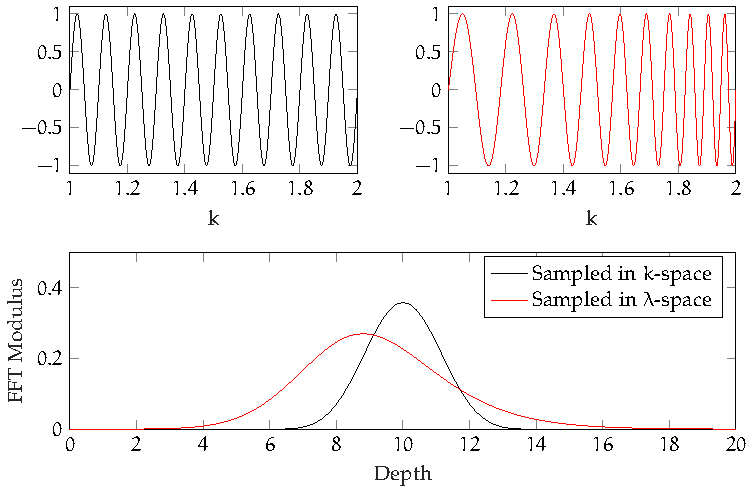
\includegraphics[width=0.95\linewidth]{gfx/tikz/fdoct-resampling}
	\caption{Interference distortion induced by linear sampling in the $\lambda$ space. }\label{fig:fdoct-resampling}
\end{figure}

\paragraph{Sensitity falloff}
A second harmful effect on the performance of these types of FD-OCT devices is the so-called \emph{Sensitivity falloff}. Sensitivity is defined as the \ac{SNR} when the sample is an ideal reflector. It's been experimentally demostrated that for increasing imaging depths, the sensitivity value drops. Such effect is illustrated in \autoref{fig:falloff}. This behaviour is due to the fact that when increasing the \ac{OPD} between reference and sample arm, the coherence function $\gamma(\Delta z)$ decreases as the two reflected signals only partially overlap, resulting in a lower signal intensity. 

\begin{figure}[bth]
	\myfloatalign
	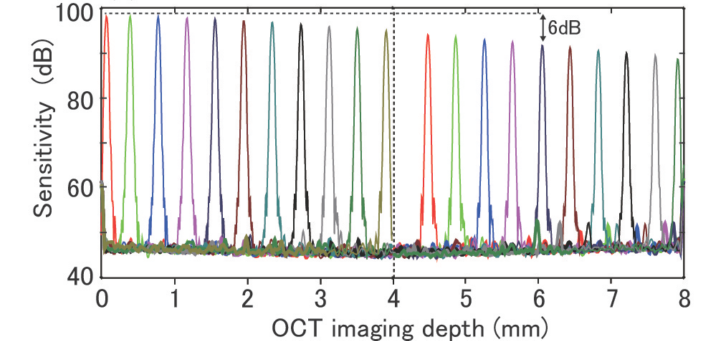
\includegraphics[width=\linewidth]{gfx/ch2/falloff}
	\caption{Sensitivity falloff in \ac{FD-OCT} systems \cite{Choi2012}.}\label{fig:falloff}
\end{figure}


An additional factor that contributes to this detrimental effect is the resolution of the photodetector arrays used to acquire the interference signal. As previously explained, higher imaging depths correspond to higher spectrum modulation frequencies. If the number of pixel $N$ of, e.g., a \ac{CCD} camera is not sufficiently high, the higher frequency components will be undersampled, reducing the range of visibility. Beam diameter and camera's pixel size also influence the loss of sensitivity. 

\paragraph{Imaging Artifacts} The massive gain in acquisition rate that comes from detecting the whole imaging range in a single shot is offset by the introduction of different artifacts in the reconstructed A-scans. The interference pattern acquired by the photodetectors array is comprised of three terms:
\begin{enumerate}
	\item \emph{DC component}. All the reflected replicas of the impinging signal coming from the sample contribute to a constant DC offset in the interference signal. These are equivalent to the non-interfering terms in the Michelson interferometer formula. When Fourier-transformed, they will appear as a reflector positioned at the very start of the imaging range, where the \ac{OPD} is close to zero. A simple solution to this problem is to compute and subtract the average value of the spectrum before applying the Fourier Transform.
	
	\item \emph{Cross-Correlation terms}. These are the interference terms that arise from the correlation between the reference signal and the reflections coming from the sample arm. As previously discussed, they contain the information required to reconstruct the reflectivity profile of the sample. 
	
	\item \emph{Auto-Correlation terms}. They result from the interference between reflectors in the sample that are less than a coherence length apart. 
\end{enumerate}


\begin{figure}[hbt]
	\myfloatalign
	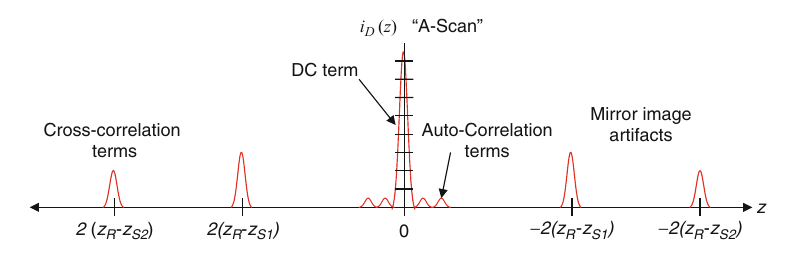
\includegraphics[width=\linewidth]{gfx/ch2/fdoct-artifacts}
	\caption{\cite{Drexler2015}}\label{fig:artifacts}
\end{figure}

These components are visible in \autoref{fig:artifacts}, who depicts the Fourier Transform of the interference signal generated by two reflectors. A further issue that is highlighted by this plot is the presence of the so called \emph{complex conjugate artifacts}, or mirror image artifacts. This phenomenon arises from the Fourier Transformation of a real signal, which will have the property of Hermitian simmetry (even modulus and odd phase). This means that \ac{FD-OCT} techniques cannot differentiate between positive and negative frequencies, or equivalently, between a sample placed before or after the zero \ac{OPD} position. 

The easiest way to deal with this problem is to simply drop one half of the acquired A-scan, effectively halving the maximum imaging depth of the system. Mirror artifacts will still appear in the image if the sample is too close to the scanning lens and crosses the zero \ac{OPD} position, which is fixed by the reference mirror. The part of the sample which is in the "negative" \ac{OPD} range will appear flipped and superimposed to the other part of the sample. This effect is illustrated in \autoref{fig:artifacts-mirror}, in which the scanning lens is progressively moved forward, closer to the patient's retina. 

Different methods to solve this issue and restore the full imaging range have been proposed, including complex-signal detection schemes using 3x3 fiber couplers \cite{Sarunic2005}, heterodyne detection \cite{Davis2005} and phase-shifting techniques \cite{Tao2007} using either \acp{PZT} or \acp{EOM}. 

\begin{figure}[bth]
	\myfloatalign
	{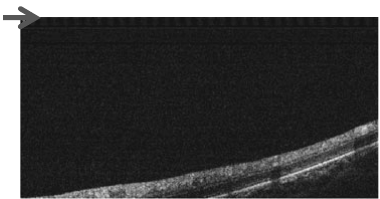
\includegraphics[width=.45\linewidth]{gfx/ch2/a}} \hspace{0.3cm}
    {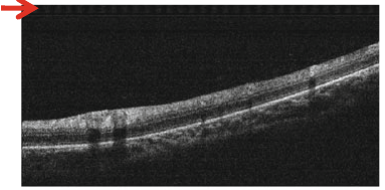
\includegraphics[width=.45\linewidth]{gfx/ch2/b}} \\[0.5cm]
	{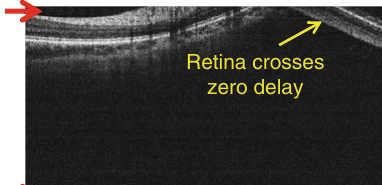
\includegraphics[width=.45\linewidth]{gfx/ch2/c}} \hspace{0.3cm}
	{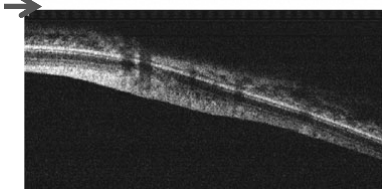
\includegraphics[width=.45\linewidth]{gfx/ch2/d}}
	\caption{Complex conjugate artifacts in \ac{SD-OCT}.}\label{fig:artifacts-mirror}
\end{figure}




\subsection{Swept-Source OCT}
\acf{SS-OCT}, also known as \ac{OFDI}, is a \ac{FD-OCT} technique that employs a narrow-bandwidth frequency-swept laser as an optical source. The introduction of tunable sources simplifies the detection scheme, removing the need for diffraction gratings and photodetector arrays. Ideally, a swept-source laser for \ac{SS-OCT} should present a frequency sweep that is linear, i.e, the istantaneous optical frequency should be expressed as
\begin{equation}\label{eq:frequency-sweep-linear}
	f(t) = f_0 + \delta f \cdot t,
\end{equation}
where $\delta f$, typically measured in Terahertz per microsecond, is the sweep rate of the source. If this requirement is satisfied, the intensity at the ouput of the interferometer when the sample is a sigle reflector positioned at the depth $d = \Delta z/2$, can be expressed as
\begin{equation}
	I(t) = I_1 + I_2 + 2\sqrt{I_1I_2}\cos\left( 2\pi \Delta f  t\right)\,
\end{equation}
where 
\begin{equation}
	\Delta f = \delta f \cdot \Delta t = \delta f \cdot \frac{\Delta z}{c} = \delta f \cdot \frac{d}{2c},
\end{equation}

 called the \emph{beat frequency}, is linearly dependant on the depth of the reflector. When the reflector is replaced by a real sample, multiple beat frequencies arise in the photodetector's current and the reflectivity profile can be reconstructed with a Fourier Transform. This technique is equivalent to \ac{SD-OCT}, with the key difference that the frequency sweep enables the detection as a function of time through a simple photodetector, while the diffraction grating spatially separates the different wavelengths and directs them to a detector array.


\begin{figure}[hbt]
	\myfloatalign
	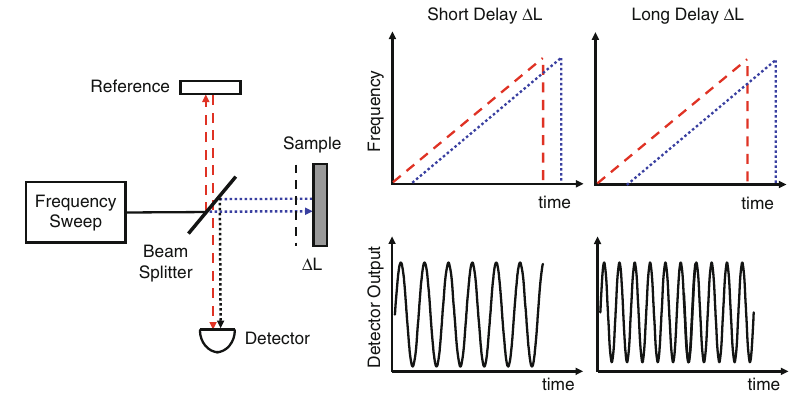
\includegraphics[width=\linewidth]{gfx/ch2/ssoct}
	\caption{\cite{Drexler2015}}\label{fig:ssoct}
\end{figure}

\subsubsection{Sweep nonlinearity}
A tunable laser generally consists of a gain medium, typically a \ac{SOA}, a tunable wavelength filter and a laser cavity that supports a large bandwidth. The frequency-sweep is achieved by controlling the tunable filter through electrical signals to select the desired wavelength. \autoref{fig:sslaser} shows the diagram of a Axsun swept source in which frequency tuning is achieved by tilting a \ac{MEMS} mirror at the end of a Fabry-Perot filter. Rapidly changing the selected wavelength can affect the linearity frequency sweep, contributing to a nonlinear term in \autoref{eq:frequency-sweep-linear}, which then becomes

\begin{equation}
	f(t) = f_0 + \delta f \cdot t + \eta (t),
\end{equation}

where $\eta(t)$ contains the aforementioned nonlinearities. If the detector's output is digitized with a uniform clock rate, a similar effect to that described for \ac{SD-OCT} systems can arise (\autoref{fig:fdoct-resampling}), resulting in a non-linear sampling in the $k$-space. Consequently, distortions in the acquired A-scans can appear, hindering the image quality. A resampling of the acquired signal is then required in order to linearize the frequency sweep, adding to the total computational cost and possibly reducing the acquisition rate of the system. 


\begin{figure}[hbt]
	\myfloatalign
	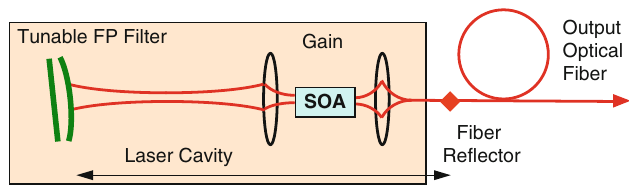
\includegraphics[width=0.7\linewidth]{gfx/ch2/sslaser}
	\caption{Frequency-swept optical source by Axsun \cite{Drexler2015}.}\label{fig:sslaser}
\end{figure}

\subsubsection{k-clocking}

While in \ac{SD-OCT} the resampling step is the only possible solution for this issue, \ac{SS-OCT} enables a hardware approach through a non-uniform clocking of the \ac{DAQ} device. This is accomplished by extracting a clock signal, called \emph{k-clock}, by means of an unbalanced \acf{MZI} which detects the frequency-sweep and generates a sinusoidal signal with a variable frequency. This approach removes the need for the computationally-intensive resampling step, but requires special \ac{DAQ} devices that can handle external clocks with a wide range of frequencies and duty cycles, which are generally more expensive.  

\subsubsection{Acquisition rate}

The acquisition speed of \ac{SS-OCT} systems is dictated by the source sweep repetition rate, that is, the frequency at which the source is able to sweep the entire bandwidth. This parameter is determined by the laser cavity length. In fact, for a given frequency, the spontaneous emission has to build up in order to reach a saturation limit to be correctly amplified by the active region. Shorter cavities with a smaller round-trip generally guarantee higher repetition rates than longer cavities. Novel swept-source designs enable acquisition speeds in the order of 100,000 A-scans per second, with \ac{FDML} and \acp{VCSEL} reaching repetition rates above 500 kHz. These high rates make \ac{SS-OCT} the primary candidate for real-time 3D visualization of \emph{in vivo} samples, where motion artifacts could hinder image quality. This is possible because the detection schemes is no longer the bottleneck like in \ac{SD-OCT}, where the slow camera response times limited the overall rate of the system. 

\subsubsection{Axial resolution}
Just like in the case of \ac{SD-OCT}, the axial resolution depends on the tuning range of the source, $\Delta \lambda$. The tuning range is defined as the \ac{FWHM} of the spectrum. In the case of a Gaussian spectrum, the axial resolution, defined as the \ac{FWHM} of the reflection peak generated by a perfect reflector, is given by
\begin{equation}\label{eq:ss-axial-resolution}
	\delta z \simeq 0.75 \cdot \frac{\lambda_0^2}{\Delta \lambda},
\end{equation}
where $\lambda_0$ is the central wavelength of operation, which is chosen based on the application (1060 nm for Ophtalmology, 1300 nm for tissue imaging). 

\subsubsection{Imaging range}
Imaging range of \ac{SS-OCT} systems is, like other \ac{FD-OCT} schemes, limited by the coherence length of the source, which we have previously defined as the \ac{OPD} at which the visibility of the interference fringes drops to 0.5. This parameter is controlled by the istantaneous linewidth of the source $\delta \lambda$ by the following equation:
\begin{equation}
	l_c \approx 0.44 \frac{\lambda_0^2}{\delta \lambda}.
\end{equation}

As with \ac{SD-OCT}, complex conjugate artifacts typically limit the imaging range to be half of the coherence length. 

When using a $k$-clock to acquire A-scans, the imaging range is also dependant on the path difference of the \ac{MZI}'s arms, which has to be 4 times the maximum imaging depth, $d_{max}$. A factor of 2 is needed because a reflector positioned at $d_{max}$ will have \ac{OPD} equal to $\Delta z = 2d_{max}$ with respect to the reference mirror. The other factor of 2 is needed to satisfy Nyquist's criterion, so that the $k$-clock will have a maximum frequency that is 2 times the beat frequency generated by the reflector at $d_{max}$. 

\subsubsection{Balanced detection}
The use of simple photodetectors instead of more complex setups involving diffraction gratings and prisms allows for a dual balanced detection scheme. By collecting the reference and sample signals through a circulator and feeding them to a 3 dB fiber coupler, two interference signals can be obtained. A balanced detector can then subtract the common DC component and the excess noise while adding the interference term. This detection scheme has been proved to be more efficient than a simple Michelson interferometer. A complete \ac{SS-OCT} scheme with dual balanced detection and external $k$-clock is illustrated in \autoref{fig:ssoct-scheme}.

\begin{figure}[hbt]
	\myfloatalign
	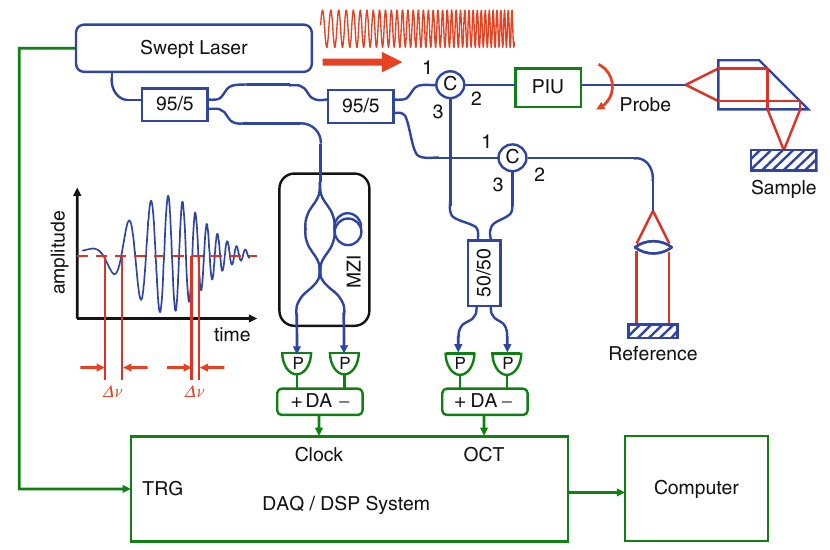
\includegraphics[width=\linewidth]{gfx/ch2/ssoct-scheme}
	\caption{Frequency-swept optical source by Axsun \cite{Drexler2015}.}\label{fig:ssoct-scheme}
\end{figure}



\begin{figure}[bth]
\myfloatalign
\subfloat[Asia personas duo.]
{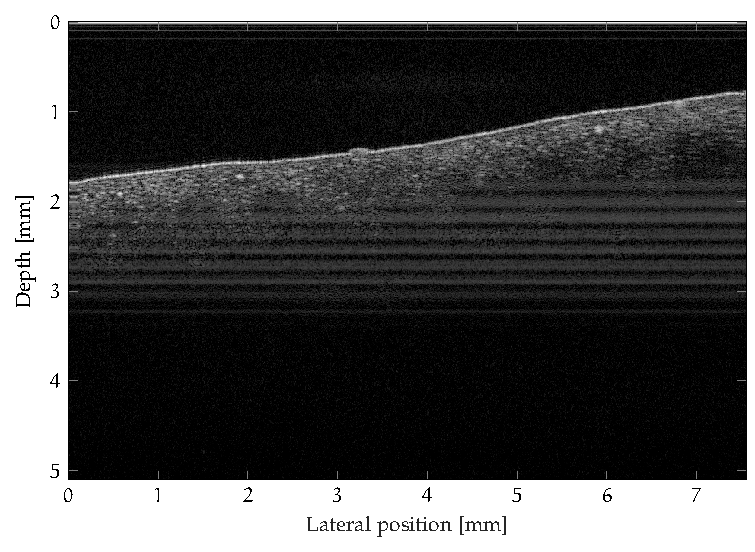
\includegraphics[width=.45\linewidth]{gfx/tikz/axsun/banana-peel}} \quad
\subfloat[Pan ma signo.]
{\label{fig:banan-peel}
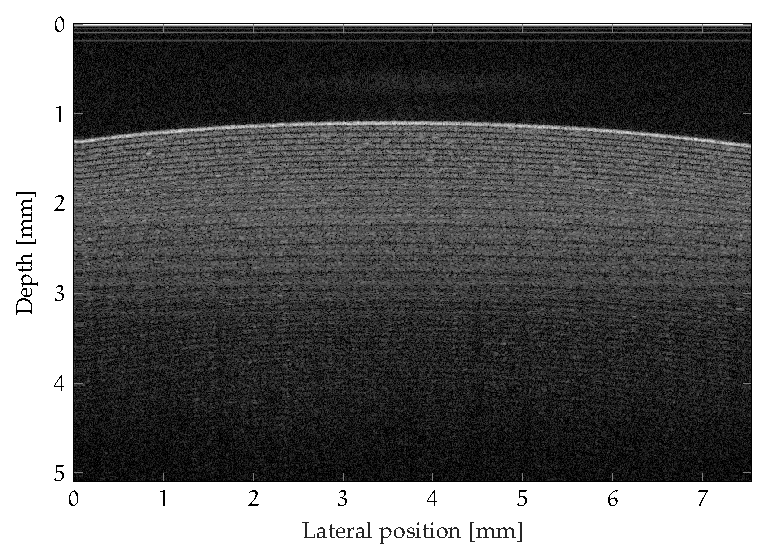
\includegraphics[width=.45\linewidth]{gfx/tikz/axsun/tape}} \\
\subfloat[Methodicamente o uno.]
{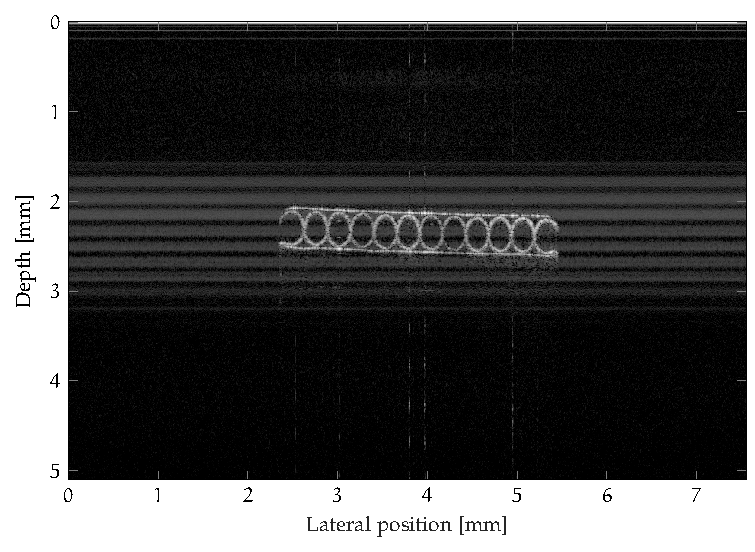
\includegraphics[width=.45\linewidth]{gfx/tikz/axsun/nastro}} \quad
\subfloat[Titulo debitas.]
{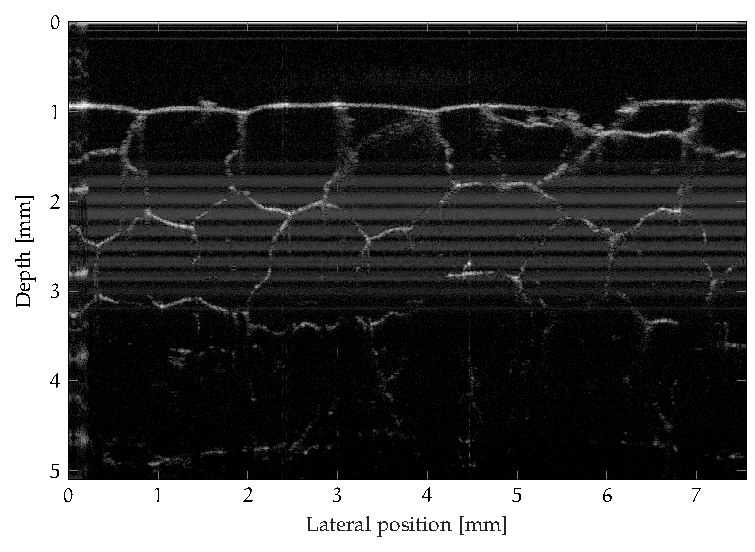
\includegraphics[width=.45\linewidth]{gfx/tikz/axsun/spugna-1}}
\caption{Tu duo titulo debitas latente.}\label{fig:example}
\end{figure}
